\chapter{Validierung}
Mit der Implementierung und Durchführung der in \autoref{Anwendungsszenarien} beschriebenen Szenarien wird das in \autoref{Konzept} erstellte Konzept validiert.

TODO

Die folgenden Abbildungen zeigen die Ergebnisse der Paketanalyse mit der vorhandenen \textit{Security Policies} "`none"'. Der \ac{OPC UA} Client des Containers "`control"', welcher die Liste der im Netzwerk vorhandenen \ac{OPC UA} Server abfrägt besitzt die \ac{IP}-Adresse 172.18.0.6, der Container des Discovery Servers die \ac{IP}-Adresse 172.18.0.2. In \autoref{Analyse:opcua-secure-none-req} ist der Request des Control Containers zum Aufbau eines \textit{Secure Channel} dargestellt. Die verwendete \textit{Security Policy} ist im Bereich "`SecurityPolicyUri"' des \ac{OPC UA} Protokolls beschrieben. In \autoref{Analyse:opcua-secure-none-res} ist die Antwort des \ac{OPC UA} Discovery Servers im \textit{Secure Channel} dargestellt. 

\begin{figure}[h]
  \centering
  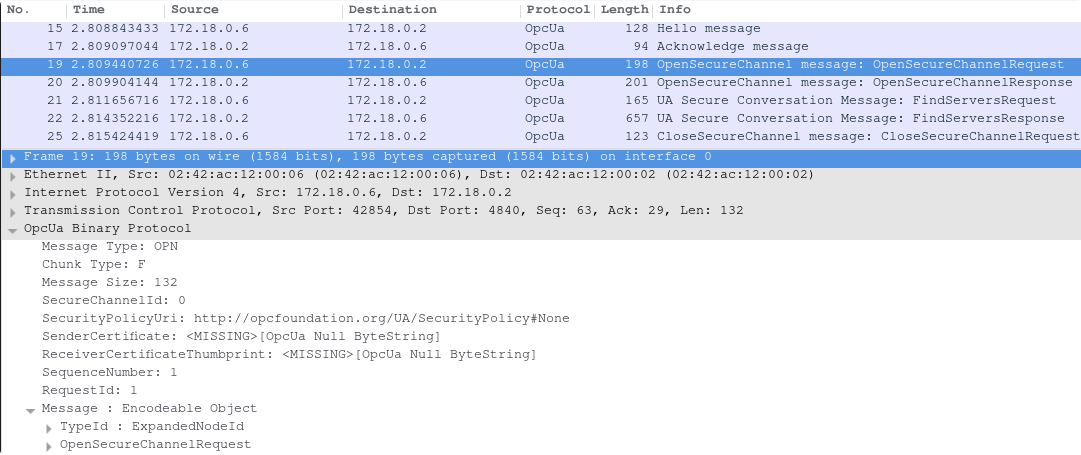
\includegraphics[width=15cm]{opcua-secure-none-req}
  \caption{Paketanalyse OPC UA - Client Request bei Sicherheitsprofil "none"} 
  \label{Analyse:opcua-secure-none-req}
\end{figure}

\begin{figure}[h]
  \centering
  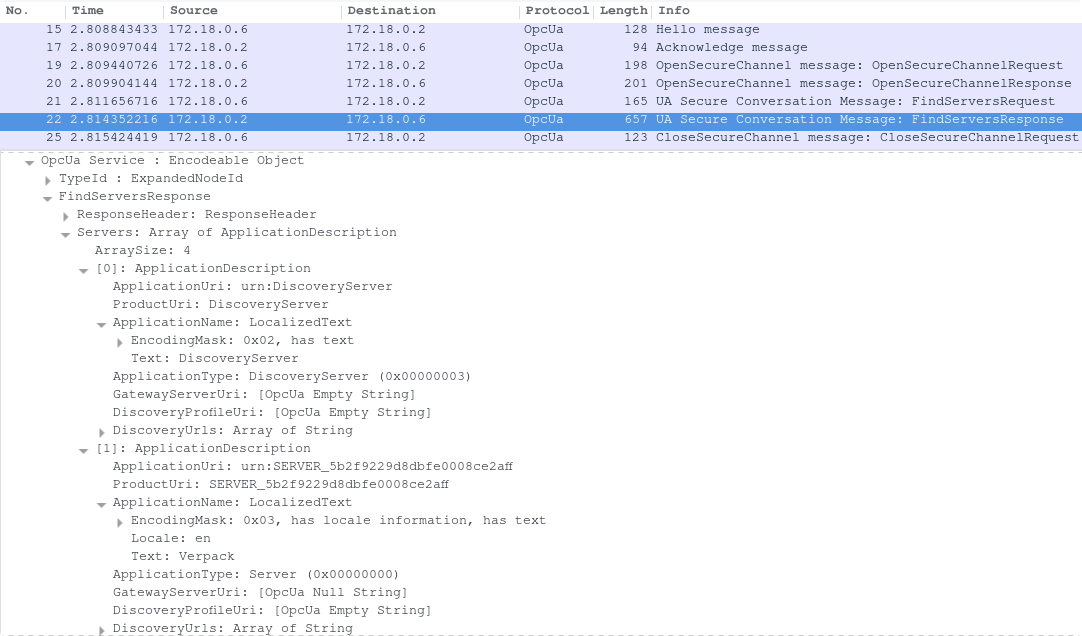
\includegraphics[width=15cm]{opcua-secure-none-res}
  \caption{Paketanalyse OPC UA - Server Response bei Sicherheitsprofil "none"} 
  \label{Analyse:opcua-secure-none-res}
\end{figure}

\clearpage

Es ist zu erkennen, dass die Kommunikation, obwohl der \textit{Secure Channel} genutzt wird, nicht verschlüsselt ist. Die Endpunkte sowie deren Adressen und bereitgestellte Methoden können aus den Paketen ausgelesen werden.

Im Folgenden wird erneut das Abfragen des Control Containers aller im Netzwerk vorhandenen Endpunkte beim Discoveryserver beschrieben, jedoch wird das Sicherheitsprofil "Basic256Sha256" mit dem \textit{MessageSecurityMode} "SIGNANDENCRYPT" genutzt. Der \ac{OPC UA} Client besitzt die \ac{IP}-Adresse 172.18.0.7. Der Discoveryserver weiterhin die Adresse 172.18.0.2. \autoref{Analyse:opcua-secure-sha-req} zeigt den Request, \autoref{Analyse:opcua-secure-sha-res} die verschlüsselte Response im \textit{Secure Channel}.

\begin{figure}[h]
  \centering
  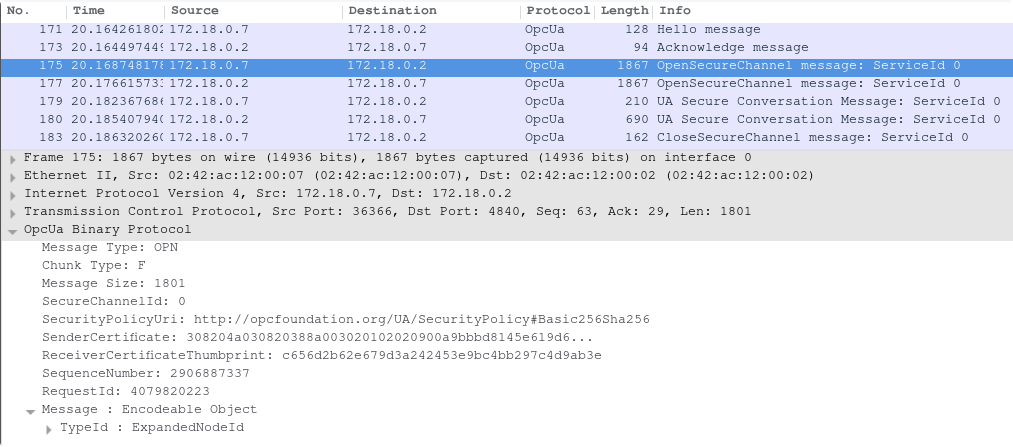
\includegraphics[width=15cm]{opcua-secure-sha-req}
  \caption{Paketanalyse OPC UA - Client Request bei Sicherheitsprofil "Basic256Sha256" und MessageSecurityMode "SIGNANDENCRYPT"} 
  \label{Analyse:opcua-secure-sha-req}
\end{figure}

\begin{figure}[h]
  \centering
  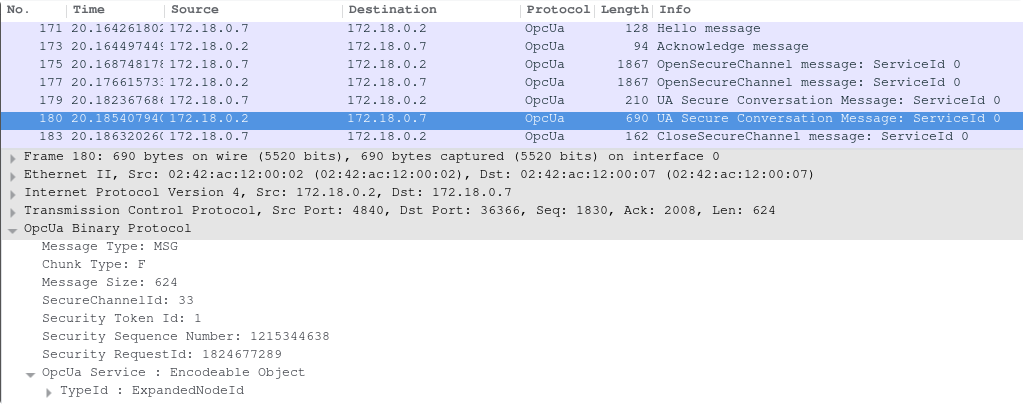
\includegraphics[width=15cm]{opcua-secure-sha-res}
  \caption{Paketanalyse OPCUA - Server Response bei Sicherheitsprofil "Basic256Sha256" und MessageSecurityMode "SIGNANDENCRYPT"} 
  \label{Analyse:opcua-secure-sha-res}
\end{figure}

\clearpage

Es ist zu erkennen, dass der gesamte Netzwerkverkehr im \textit{Secure Channel} durch den Algorithmus SHA256 verschlüsselt wurde.